\documentclass[tikz]{standalone}
\usepackage{tikz}

\begin{document}

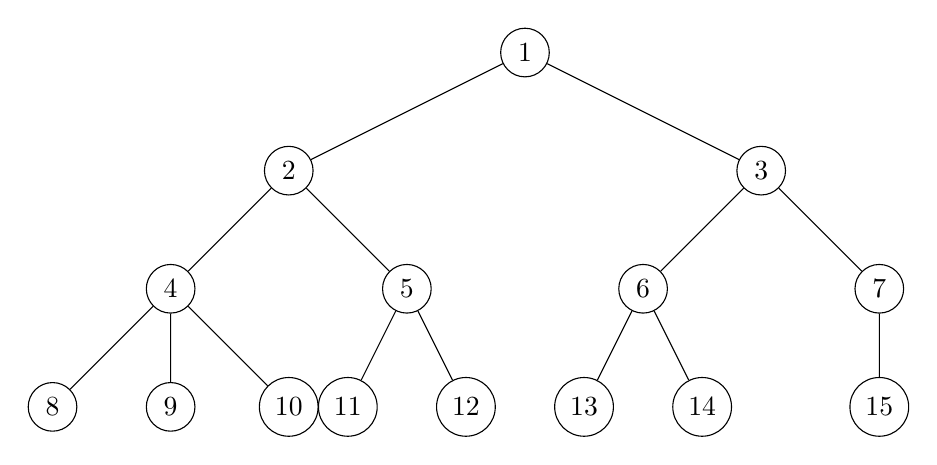
\begin{tikzpicture}[level distance=1.5cm,
  level 1/.style={sibling distance=6cm},
  level 2/.style={sibling distance=3cm},
  level 3/.style={sibling distance=1.5cm}]
  
  \node[draw, circle] {1}
    child { node[draw, circle] {2} 
      child { node[draw, circle] {4} 
        child { node[draw, circle] {8} }
        child { node[draw, circle] {9} }
        child { node[draw, circle] {10} } % Drittes Blatt hinzugefügt
      } 
      child { node[draw, circle] {5}
        child { node[draw, circle] {11} }
        child { node[draw, circle] {12} }
      }
    }
    child { node[draw, circle] {3}
      child { node[draw, circle] {6}
        child { node[draw, circle] {13} }
        child { node[draw, circle] {14} }
      }
      child { node[draw, circle] {7}
        child { node[draw, circle] {15} }
        % Hier wurde ein Knoten entfernt, um die Gesamtzahl der Knoten auf 15 zu halten
      }
    };
\end{tikzpicture}

\end{document}
